\subsection{Catálogo de actores}
	\begin{table}[h]
\centering
\begin{tabular}{|c|l|l}
\cline{1-2}
\textbf{ACT-0001}    & \multicolumn{1}{|c|}{\textbf{Usuario}}                                                                                                                    &  \\ \cline{1-2}
\textbf{Versión}     & 1.0 (20/03/2014)                                                                                                                                            &  \\ \cline{1-2}
\textbf{Fuente}      & Epresa21                                                                                                                                                    &  \\ \cline{1-2}
\textbf{Descripción} & \begin{tabular}[c]{@{}c@{}}Este actor representa a cada uno de los usuarios de la aplicación \\ de recogida de enseres.\end{tabular}                        &  \\ \cline{1-2}
\textbf{Comentario}  & \begin{tabular}[c]{@{}c@{}}previa petición de los mismos al teléfono 956 880 884 o bien \\ solicitud web mediante portal web del ayuntamiento.\end{tabular} &  \\ \cline{1-2}
\end{tabular}
\caption{ACT-0001 Usuario}
\end{table}
	\begin{table}[h]
\centering
\begin{tabular}{|c|l|l}
\cline{1-2}
\textbf{ACT-0002}    & \multicolumn{1}{|c|}{\textbf{Operador}}                                                                                                                                                                                          &  \\ \cline{1-2}
\textbf{Versión}     & 1.0 (20/03/2014)                                                                                                                                                                                                                 &  \\ \cline{1-2}
\textbf{Fuente}      & Epresa21                                                                                                                                                                                                                         &  \\ \cline{1-2}
\textbf{Descripción} & \begin{tabular}[c]{@{}c@{}}Este actor representa al operador que consulta desde la sede de la\\ \\ empresa las peticiones de recogida realizadas y realiza informes\\ mensuales cuando lo solicita el ayuntamiento.\end{tabular} &  \\ \cline{1-2}
\textbf{Comentario}  & \begin{tabular}[c]{@{}c@{}}Dicho usuario pertenece a la localidad en la que se proporciona\\ el servicio.\end{tabular}                                                                                                           &  \\ \cline{1-2}
\end{tabular}
\caption{ACT-0002 Operador}
\end{table}
	
\subsection{Requisitos funcionales}
\subsubsection*{Casos de uso del sistema}
	\begin{figure}[H]
	\centering
 	   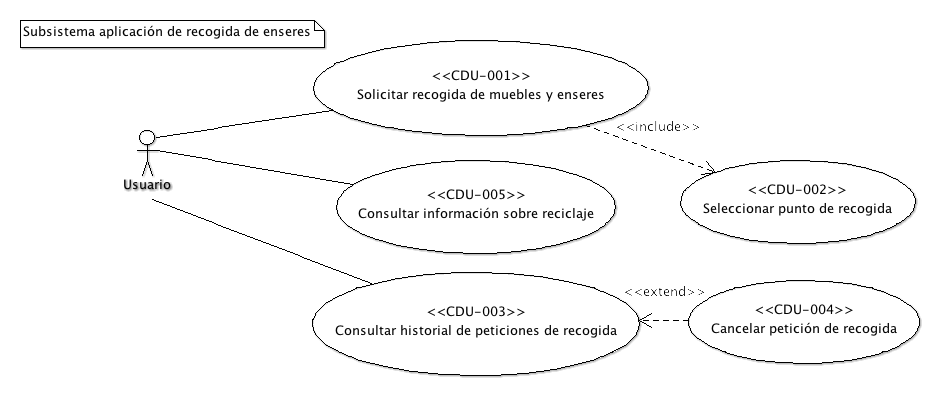
\includegraphics[scale=0.50]{diagramaCU1.png} 
  	  \caption{Diagrama UML del Subsistema aplicación de recogida de muebles y enseres.}
	\end{figure}	
	% CDU-001: Solicitar recogida de muebles y ensere
\begin{longtable}{p{2.5cm}  p{14cm}}
\caption*{\textbf{CDU-001: Solicitar recogida de muebles y enseres}} \\
\hline
\textbf{Versión} & 1.0 (26/03/2014) \\
\textbf{Fuentes} & Apresa21 \\
\textbf{Dependencias} & OBJ-001 CDU-002 \\
% Descripción del caso de uso
\textbf{Descripción} & El sistema deberá comportarse tal como se describe en el siguiente caso de uso cuando \textit{un usuario desee solicitar la recogida de uno o varios muebles y enseres.} \\
\textbf{Frecuencia esperada} & 10 veces al día \\
\textbf{Importancia} & Vital  \\
\textbf{Comentarios} &- \\
\end{longtable}

\textbf{Secuencia Normal} 
\begin{enumerate}
	\item[1.] El actor \textit{Usuario (ACT-0001)} solicita al sistema la recogida de uno o varios muebles y enseres.
	\item[2.] El \textit{Sistema} solicita al \textit{Usuario (ACT-0001)} que indique qué tipo de mueble o enser quiere depositar para su recogida, así como el volumen de dicho objeto.
	% Excepción en el paso 3
	\item[3.] El actor \textit{Usuario (ACT-0001)} indica qué tipo de mueble o enser va a depositar así como las características del mismo (Repetir este paso hasta que se hayan incluido todos los objetos que el actor \textit{Usuario (ACT-0001)} desea depositar para su posterior recogida).
	\item[4.] Seleccionar punto donde se depositarán los muebles y enseres para su posterior recogida. \textbf{Include (Seleccionar punto de recogida)}

	\item[5.] El \textit{Sistema} comprueba la primera fecha disponible para registrar la cita para recogida de los muebles y enseres.
	% Excepción en el paso 6
	\item[6.] El \textit{Sistema} comprueba si se han solicitado más del número máximo de objetos al día que se pueden recoger. Se han solicitado menos del número máximo de objetos por usuario al día que se pueden solicitar para que sean recogidas. Adicionalmente se comprueba si es posible dar respuesta a la recogida de objetos dentro del cupo de recogida 	diaria para dicha fecha. Se comprueba que es posible recoger todos los enseres en el mismo día.
	\item[7.] El \textit{Sistema} muestra al usuario las instrucciones que debe seguir para depositar los muebles y enseres. Una vez mostradas muestra la fecha y localización de la recogida y solicita confirmación.
	\item[8.] El actor \textit{Usuario (ACT-0001)} visualiza todas las instrucciones y confirma la recogida de muebles y enseres.
	\item[9.] El \textit{Sistema} registra en el sistema la fecha de recogida y el número de enseres, así como la ubicación.
	\item[10.] El \textit{Sistema} muestra al usuario una confirmación a la solicitud de recogida de muebles y enseres con la fecha y lugar donde serán recogidos.
\end{enumerate} 

\textbf{Postcondición: } 
 Se registra la solicitud de recogida de muebles y enseres con la ubicación y fecha(s).\\

\textbf{Excepciones} 
\begin{enumerate}
\item[*a.] El actor \textit{Usuario (ACT-0001)} cancela el proceso de solicitud de recogida de muebles y enseres.
	\begin{enumerate}
		\item[1.] El Sistema cancela el registro de la solicitud de recogida de muebles y enseres.
	\end{enumerate}
\item[3a.] El actor \textit{Usuario (ACT-0001)} desea solicitar la recogida de más de un mueble o enser.
	\begin{enumerate}
		 \item[1.] El actor \textit{Usuario (ACT-0001)} vuelve a indicar que tipo de mueble o enser va a depositar así como las características del mismo.
		 \item[2.] EL \textit{Sistema} incluye el objeto en el listado de muebles y enseres que el usuario desea que sean recogidos para reciclar.
		 \item[3.] EL \textit{Sistema} comprueba si se ha superado el máximo número de muebles y enseres que se pueden recoger por usuario al día. En caso afirmativo muestra un mensaje al usuario informando que el máximo número de objetos que se recogen por día es ese y que la recogida se hará en varias jornadas.
	\end{enumerate}
\item[3b.] El actor \textit{Usuario (ACT-0001)} desea solicitar la recogida de un mueble o enser que no esta en el listado de productos recogidas y cuyas características no se pueden indicar.
	\begin{enumerate}
		\item[1.] El \textit{Sistema} informa al usuario que debe ponerse en contacto con el número de teléfono de la empresa municipal (Se finaliza el caso de uso).
	\end{enumerate}	
\item[6a.] El \textit{Sistema} comprueba que no es posible dar servicio en un solo día a la petición del usuario al sobrepasar el número de objetos que pueden recogerse en un día o en el primer día disponible.
	\begin{enumerate}
		\item[1.] El Sistema organiza la recogida en varios días teniendo el cuenta el máximo número de objetos que se recogen por día y usuario y el número de objetos que se van a recoger en la primera fecha disponible. Vuelve al paso 11.
	\end{enumerate}
\item[9a.] El \textit{Sistema} no puede registrar  en el sistema la fecha de recogida y el número de enseres, así como la ubicación.
	\begin{enumerate}
		\item[1.] El \textit{Sistema} informa de que no ha sido posible resolver la solicitud del usuario y que debe ponerse en contacto con el Teléfono de contacto de la empresa de recogida de muebles y enseres.
	\end{enumerate}
\end{enumerate}

	% CDU-002: Seleccionar punto de recogida
\begin{longtable}{p{2.5cm}  p{14cm}}
\caption*{\textbf{CDU-002: Seleccionar punto de recogida}} \\
\hline
\textbf{Versión} & 1.0 (26/03/2014) \\
\textbf{Fuentes} & Apresa21 \\
\textbf{Dependencias} & OBJ-001 CDU-001 \\
% Descripción del caso de uso
\textbf{Descripción} & El sistema deberá comportarse tal como se describe en el siguiente caso de uso cuando \textit{haya que seleccionar una ubicación donde el usuario depositará sus muebles y enseres para que posteriormente sean recogidos por el camión de la empresa de reciclaje.} \\
\textbf{Frecuencia esperada} & 10 veces al día \\
\textbf{Precondición} & El terminal móvil del usuario dispone de tecnología GPS funcional y con cobertura. \\
\textbf{Importancia} & Vital  \\
\textbf{Comentarios} & Se establece como distancia máxima del domicilio del cliente 300 metros del punto de depósito de los mueble y enseres. Para distancias mayores se remite al usuario a contactar vía telefónica con la empresa de recogida de muebles y enseres. \\
\end{longtable}

\textbf{Secuencia Normal} 
\begin{enumerate}
	\item[1.] El \textit{Sistema} solicita al usuario si desea introducir su dirección manualmente o bien ser geolocalizado mediante el sistema de localización GPS del propio terminal móvil.
	% Excepción en el paso 2
	\item[2.] El actor \textit{Usuario (ACT-0001)} introduce indica que desea introducir manualmente el punto de recogida, introduce su calle y número.
	% Excepción en el paso 3
	\item[3.] El \textit{Sistema} comprueba si la localización corresponde al término municipal donde se oferta el servicio de recogida de muebles y enseres.
	\item[4.] El \textit{Sistema} comprueba si el punto de recogida se encuentra a menos de 300 metros del domicilio del usuario y muestra al usuario el punto de recogida más cercano a su domicilio. 
	\item[5.] El \textit{Sistema} comprueba si la localización corresponde a una zona rural o una zona urbana del término municipal. Es una zona urbana. 
\end{enumerate}

\textbf{Postcondición: } 
 Se obtiene el punto donde de recogida donde el usuario depositará los muebles y enseres.\\

\textbf{Excepciones} 
\begin{enumerate}
	\item[2a.] El actor \textit{Usuario (ACT-0001)} desea emplear la localización por medio del servicio GPS de su terminal móvil.
	\begin{enumerate}
		\item[1.] El Sistema solicita al terminal móvil la ubicación GPS en la cual se encuentra en ese mismo instante.
		\item[2.] El Sistema obtiene las coordenadas del domicilio del usuario por medio del servicio de localización GPS. Vuelve al paso 3.
	\end{enumerate}
	\item[3a.] El \textit{Sistema} comprueba que la localización está fuera del término municipal donde se oferta el servicio de recogida de muebles y enseres.
	\begin{enumerate}
		\item[1.] El \textit{Sistema} informa al usuario que actualmente el servicio solo se oferte en dicho término municipal y que no es posible prestarle el servicio. Se finaliza el caso de uso.
	\end{enumerate}
	\item[4a.] El \textit{Sistema} comprueba que todos los puntos de recogida están a más de 300 metros del domicilio del usuario que solicita el servicio.
	\begin{enumerate}
		\item[1.] El \textit{Sistema} informa al usuario que debe ponerse en contacto con el número de teléfono de la empresa municipal. Se finaliza el caso de uso.
	\end{enumerate} 	
\end{enumerate} 

	% CDU-003: Consultar Historial de Peticiones de Recogida
\begin{longtable}{p{2.5cm}  p{14cm}}
\caption*{\textbf{CDU-003: Consultar Historial de Peticiones de Recogida}} \\
\hline
\textbf{Versión} & 1.0 (26/03/2014) \\
\textbf{Fuentes} & Apresa21 \\
\textbf{Dependencias} & OBJ-001 \\
% Descripción del caso de uso
\textbf{Descripción} & El sistema deberá comportarse tal como se describe en el siguiente caso de uso cuando \textit{un usuario desee consultar las peticiones de recogida de uno o varios muebles y enseres que ha solicitado anteriormente.} \\
\textbf{Frecuencia esperada} & 1 veces a la semana  \\
\textbf{Precondición} & El actor \textit{Usuario (ACT-0001)} ha realizado anteriormente una o varios solicitudes de recogida de mueble y enseres. \\
\textbf{Importancia} & Baja  \\
\textbf{Comentarios} &- \\
\end{longtable}

\textbf{Puntos de extensión:} 
borrar en 3a. \\

\textbf{Secuencia Normal} 
\begin{enumerate}
	\item[1.] El actor \textit{Usuario (ACT-0001)} desea consultar las solicitudes que ha realizado de recogida de muebles y enseres.
	\item[2.] El sistema consulta las peticiones de recogida de muebles y enseres que tiene pendiente y las que ha realizado anteriormente y las muestra por pantalla.
	\item[3] El actor \textit{Usuario (ACT-0001)} selecciona una petición para visualizar mas detalles.
\end{enumerate}

\textbf{Postcondición: } 
 Se muestran por pantalla las peticiones de recogida de muebles y enseres que ha realizado el usuario.\\

\textbf{Excepciones} 
\begin{enumerate}
	\item[3a.] El actor \textit{Usuario (ACT-0001)} desea cancelar una petición que ha solicitado y que aún está pendiente de resolución.
\end{enumerate} 	
	% CDU-004: Cancelar petición de recogida
\begin{longtable}{p{2.5cm}  p{14cm}}
\caption*{\textbf{CDU-004: Cancelar petición de recogida}} \\
\hline
\textbf{Versión} & 1.0 (26/03/2014) \\
\textbf{Fuentes} & Apresa21 \\
\textbf{Dependencias} & OBJ-001 CDU-003 \\
% Descripción del caso de uso
\textbf{Descripción} & El sistema deberá comportarse tal como se describe en el siguiente caso de uso cuando \textit{un Usuario desee cancelar una solicitud de recogida de muebles y enseres que tiene pendiente para los próximos días.} \\
\textbf{Frecuencia esperada} & 1 vez al mes  \\
\textbf{Precondición} & El actor \textit{Usuario (ACT-0001)} ha realizado anteriormente una o varios solicitudes de recogida de mueble y enseres. Dicha solicitud se realizará en una fecha posterior a la fecha del Sistema. \\
\textbf{Importancia} & Baja  \\
\textbf{Comentarios} & Sólo se cancelarán las peticiones de recogidas de enseres pendiente, con fechas posteriores a la fecha actual del Sistema. \\
\end{longtable}

\textbf{Secuencia Normal} 
\begin{enumerate}
	\item[1.] El actor \textit{Usuario (ACT-0001)} desea cancelar una petición, anteriormente seleccionada y pendiente de realizar, para que le recojan muebles y enseres.
	\item[2.] El \textit{Sistema} muestra un mensaje al usuario confirmando la eliminación de la petición de recogida de muebles y enseres.
	\item[3.] El actor \textit{Usuario (ACT-0001)} confirma su deseo de eliminar la petición.
	\item[4.] El \textit{Sistema} elimina la petición de recogida de muebles y enseres de los registros de solicitudes y actualiza el histórico de solicitudes de recogida de muebles y enseres.
\end{enumerate}
	% CDU-005: Consultar información sobre reciclaje
\begin{longtable}{p{2.5cm}  p{14cm}}
\caption*{\textbf{CDU-005: Consultar información sobre reciclaje}} \\
\hline
\textbf{Versión} & 1.0 (27/03/2014) \\
\textbf{Fuentes} & Apresa21 \\
\textbf{Dependencias} & OBJ-002 \\
% Descripción del caso de uso
\textbf{Descripción} & El sistema deberá comportarse tal como se describe en el siguiente caso de uso cuando \textit{un usuario solicita información sobre información útil sobre el reciclaje, todas sus aplicaciones, ventajas y beneficios para el medioambiente.} \\
\textbf{Frecuencia esperada} & 30 veces a la semana  \\
\textbf{Precondición} & - \\
\textbf{Importancia} & Baja  \\
\textbf{Comentarios} &- \\
\end{longtable}

\textbf{Secuencia Normal} 
\begin{enumerate}
	\item[1.] El actor \textit{Usuario (ACT-0001)} consulta información sobre el reciclaje y todas sus aplicaciones ventajas y beneficios para el medioambiente.
	\item[2.] El \textit{Sistema} muestra la información agrupada en función del tipo de residuo.
	\item[3.] El actor \textit{Usuario (ACT-0001)} elige un tipo de residuo.
	\item[4.] El \textit{Sistema} muestra la información disponible sobre dicho residuo.
\end{enumerate}	
	
	\begin{figure}[H]
	\centering
 	   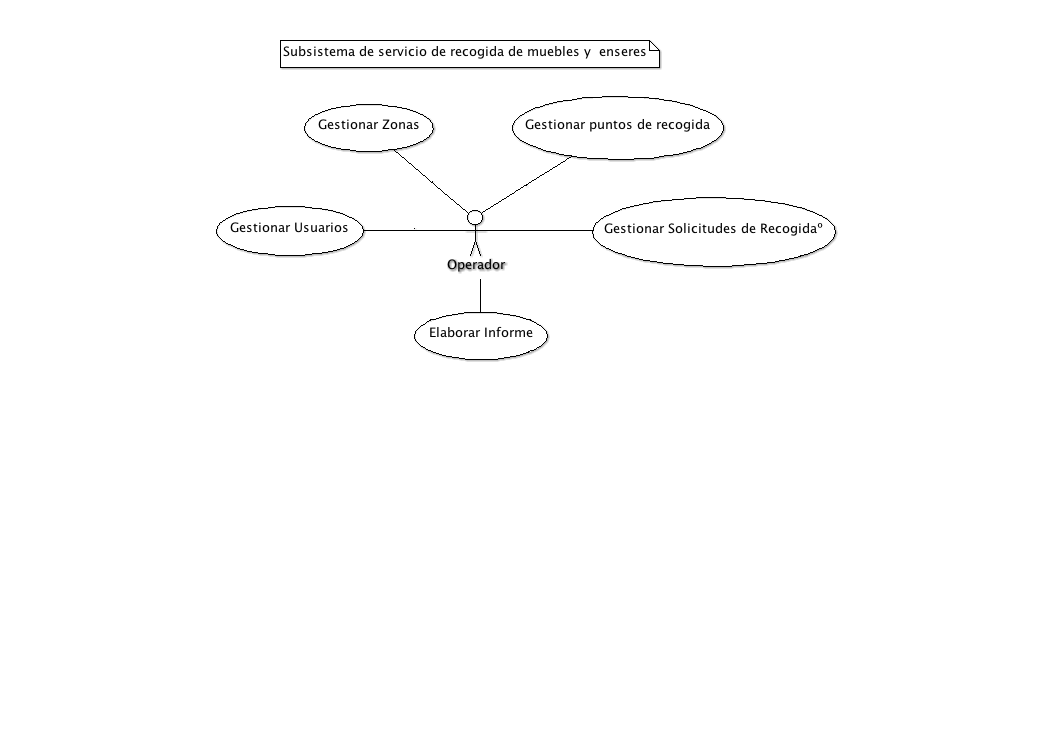
\includegraphics[scale=0.50]{diagramaCU2.png} 
  	  \caption{Diagrama UML del Subsistema de servicio de recogida de muebles y enseres.}
	\end{figure}	

\subsection{Requisitos de información}
	% Información sobre enseres
\begin{center}
\begin{longtable}{|p{80pt}|p{9cm}|}
\hline
\textbf{IRQ-001} & Información sobre Enseres \\ \hline
\textbf{Dependencias} & OBJ-001 \\ \hline
\textbf{Descripción} & El sistema deberá almacenar la información correspondiente a los Tipos de Enseres que se vayan a recoger de cara a planificar las rutas del camión. En concreto: \\ \hline
\textbf{Datos \mbox{específicos}} & 
\begin{itemize}
    \item Nombre del enser ( \textit{Identificador del objeto que se debe recoger} )
    \item Volumen ( \textit{Aproximado en metros cúbicos} )
    \item Altura ( \textit{Aproximado en metros cúbicos} )
    \item Anchura ( \textit{Aproximado en metros cúbicos} )
    \item Peso ( \textit{Aproximado en kilogramos} )
\end{itemize}\\ \hline
\caption{IRQ-001  Información sobre Enseres}
\end{longtable}
\end{center}
	% Unicidad de Enseres
\begin{center}
\begin{longtable}{|p{80pt}|p{9cm}|}
\hline
\textbf{CRQ-001} & Unicidad de Enseres \\ \hline
\textbf{Dependencias} & OBJ-001 \\ \hline
\textbf{Descripción} & La información almacenada por el sistema deberá satisfacer la siguiente restricción: todas los enseres tendrán un Nombre de enser único. \\ \hline
\caption{CRQ-001 Unicidad de Enseres}
\end{longtable}
\end{center}

	% Información sobre usuarios
\begin{center}
\begin{longtable}{|p{80pt}|p{9cm}|}
\hline
\textbf{IRQ-002} & Información sobre Usuarios \\ \hline
\textbf{Dependencias} & OBJ-001 y OBJ-003 \\ \hline
\textbf{Descripción} & El sistema deberá almacenar la información correspondiente Usuarios que solicitan la recogida de enseres. En concreto: \\ \hline
\textbf{Datos \mbox{específicos}} & 
\begin{itemize}
    \item Nombre del Usuario ( \textit{Identificador del usuario que solicita la recogida de muebles o enseres} )
    \item Apellidos del Usuario ( \textit{Sus apellidos, este campo es opcional} )
    \item Teléfono de contacto ( \textit{El número de teléfono del móvil desde el que tiene instalada la aplicación} )
    \item Identificador ( \textit{Un número que identifique al usuario de forma unívoca} )
\end{itemize}\\ \hline
\caption{IRQ-002  Información sobre Usuarios}
\end{longtable}
\end{center}
	% Unicidad de Usuarios
\begin{center}
\begin{longtable}{|p{80pt}|p{9cm}|}
\hline
\textbf{CRQ-002} & Unicidad de Usuarios \\ \hline
\textbf{Dependencias} & OBJ-001 y OBJ-003 \\ \hline
\textbf{Descripción} & La información almacenada por el sistema deberá satisfacer la siguiente restricción: todas los Usuarios tendrán un Identificador de Usuario único. \\ \hline
\caption{CRQ-002 Unicidad de Usuarios}
\end{longtable}
\end{center}
	
	% Información sobre recogidas de enseres
\begin{center}
\begin{longtable}{|p{80pt}|p{9cm}|}
\hline
\textbf{IRQ-003} & Información sobre las  Solicitudes de recogidas de muebles y enseres \\ \hline
\textbf{Dependencias} & OBJ-001 y OBJ-003 \\ \hline
\textbf{Descripción} & El sistema deberá almacenar la información correspondiente las solicitudes de recogidas de muebles de enseres. En concreto: \\ \hline
\textbf{Datos \mbox{específicos}} & 
\begin{itemize}
    \item Identificador de solicitud ( \textit{Identificador de solicitud de recogida de muebles o enseres} )
    \item Usuario solicitante ( \textit{Identificador de usuario que solicita la recogida de muebles o enseres} )
    \item Fecha ( \textit{Fecha en la que se estipula la recogida de los muebles y enseres} )
    \item Punto de recogida ( \textit{Ubicación en la que se depositarán los muebles y enseres} )
    \item Tipo de muebles y enseres depositados ( \textit{Tipo de muebles y enseres que se depositarán en el punto de recogida} )
\end{itemize}\\ \hline
\caption{IRQ-003 Información sobre las solicitudes de recogidas de muebles y enseres}
\end{longtable}
\end{center}
	% Unicidad de solicitudes de recogida de muebles y enseres
\begin{center}
\begin{longtable}{|p{80pt}|p{9cm}|}
\hline
\textbf{CRQ-003} & Unicidad de solicitudes de recogida de muebles y enseres \\ \hline
\textbf{Dependencias} & OBJ-001 y OBJ-003 \\ \hline
\textbf{Descripción} & La información almacenada por el sistema deberá satisfacer la siguiente restricción: todas los solicitudes de recogidas de muebles y enseres tendrán un Identificador de solicitud único. \\ \hline
\caption{CRQ-003 Unicidad de solicitudes de recogida de muebles y enseres}
\end{longtable}
\end{center}
	
	% Información sobre los puntos de recogida
\begin{center}
\begin{longtable}{|p{80pt}|p{9cm}|}
\hline
\textbf{IRQ-004} & Información sobre los puntos de recogida \\ \hline
\textbf{Dependencias} & OBJ-001 \\ \hline
\textbf{Descripción} & El sistema deberá almacenar la información correspondiente los puntos de recogida de muebles y enseres. En concreto: \\ \hline
\textbf{Datos \mbox{específicos}} & 
\begin{itemize}
    \item Identificador de solicitud ( \textit{Identificador de solicitud de recogida de muebles o enseres} )
    \item Zona ( \textit{Si es zona rural o zona urbana} )
    \item Posición ( \textit{localización gps del punto de recogida} )
\end{itemize}\\ \hline
\caption{IRQ-004Información sobre los puntos de recogida}
\end{longtable}
\end{center}
	
	\newpage
	\subsubsection*{Diagrama conceptual de clases UML}
	\begin{figure}[H]
	\centering
 	   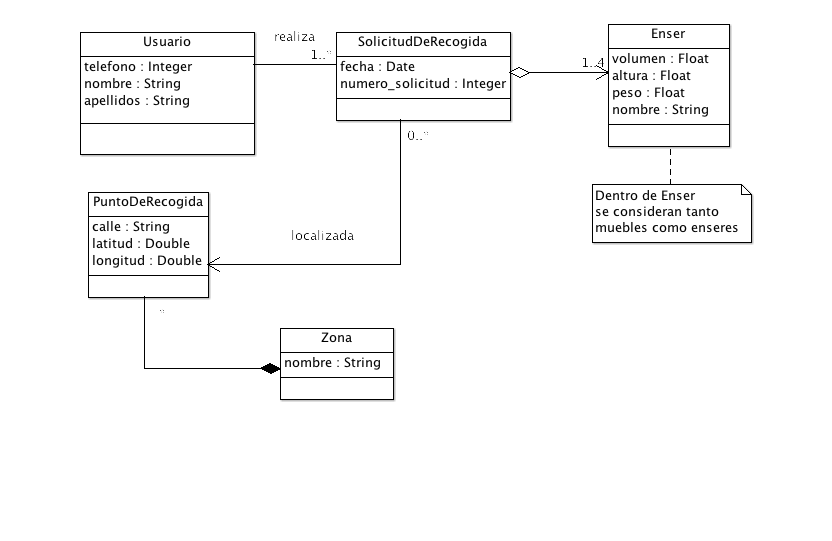
\includegraphics[scale=0.70,angle =90]{diaConceptualUML.png} 
  	  \caption{Diagrama conceptual de clases UML.}
	\end{figure}
	
	\newpage
	\subsubsection*{Tipos}
	% Tipo Usuario
	% Tipo que representa USUARIOS

\begin{longtable}{p{2.5cm}  p{14cm}}
\caption*{\textbf{TYP-001: Usuario}} \\
\hline
\textbf{Versión} & 1.0 (31/03/2014) \\
\textbf{Fuentes} & Apresa21 \\
% Descripción del Tipo
\textbf{Descripción} & Este tipo de objetos representa  \textit{los usuarios que solicitan recogida de muebles o enseres} \\
\textbf{Supertipo} & - \\
\textbf{Subtipo} & -  \\
\textbf{Comentarios} &- \\
\end{longtable}

\begin{longtable}{p{3cm}  p{12cm}}
\hline
\textbf{Atributo variable} & Usuario::teléfono \\
% Descripción del Atributo
\textbf{Descripción} & Este atributo representa  \textit{el número de teléfono del usuario} \\
\textbf{Tipo} & \textit{String} \\
\textbf{Comentarios} & Este campo se empleará para identificar al usuario. El teléfono es un teléfono de móvil. En caso de que haya alguna incidencia se contactará a este número. \\
\end{longtable}

\begin{longtable}{p{3cm}  p{12cm}}
\hline
\textbf{Atributo variable} & Usuario::Nombre \\
% Descripción del Atributo
\textbf{Descripción} & Este atributo representa  \textit{el nombre del solicitante del servicio de recogida y del titular del teléfono móvil.} \\
\textbf{Tipo} & \textit{String} \\
\textbf{Comentarios} &- \\
\end{longtable}

\begin{longtable}{p{3cm}  p{12cm}}
\hline
\textbf{Atributo variable} & Usuario::Apellidos \\
% Descripción 
\textbf{Descripción} & Este atributo representa  \textit{los apellidos del solicitante del servicio de recogida y titular del teléfono móvil.} \\
\textbf{Tipo} & \textit{String} \\
\textbf{Comentarios} & Este campo es opcional \\
\end{longtable}

\begin{longtable}{p{3cm}  p{12cm}}
\hline
\textbf{Expresión de invariante} & Usuario de teléfono \\
% Descripción 
\textbf{Descripción} & No puede haber Usuarios con el mismo teléfono en el Sistema. \\
\textbf{Comentarios} & - \\
\end{longtable}

	% Tipo SolicitudRecogida	
	% Tipo que representa SOLICITUDES DE RECOGIDA

\begin{longtable}{p{2.5cm}  p{14cm}}
\caption*{\textbf{TYP-002: SolicitudRecogida}} \\
\hline
\textbf{Versión} & 1.0 (31/03/2014) \\
\textbf{Fuentes} & Apresa21 \\
\textbf{Descripción} & Este tipo de objetos representa  \textit{la solicides de recogidas de muebles y enseres realizadas por los usuarios} \\
\textbf{Supertipo} & - \\
\textbf{Subtipo} & -  \\
\textbf{Comentarios} &- \\
\end{longtable}

% Atributos
\begin{longtable}{p{3cm}  p{12cm}}
\hline
\textbf{Atributo variable} & SolicitudRecogida::fecha \\
\textbf{Descripción} & Este atributo representa  \textit{la fecha en la cual se establece la solicitud de recogida.} \\
\textbf{Tipo} & \textit{String} \\
\textbf{Comentarios} & - \\
\end{longtable}

\begin{longtable}{p{3cm}  p{12cm}}
\hline
\textbf{Atributo variable} & SolicitudRecogida::numeroSolicitud \\
\textbf{Descripción} & Este atributo representa  \textit{el número de solicitud.} \\
\textbf{Tipo} & \textit{Natural} \\
\textbf{Comentarios} & Este atributo es identifica y sirve para contabilizar el número de solicitudes realizadas. \\
\end{longtable}

% Invariantes
\begin{longtable}{p{3cm}  p{12cm}}
\hline
\textbf{Expresión de invariante} & SolicitudRecogida::UnicidadnumeroSolicitud \\
\textbf{Descripción} &  \textit{No puede haber dos solicitudes de recogida con el mismo número} \\
\textbf{Comentarios} & -\\
\end{longtable}
	
	% Tipo PuntosDeRecogida	
	% Tipo que representa PUNTOS DE RECOGIDA

\begin{longtable}{p{2.5cm}  p{14cm}}
\caption*{\textbf{TYP-003: puntoRecogida}} \\
\hline
\textbf{Versión} & 1.0 (01/04/2014) \\
\textbf{Fuentes} & Apresa21 \\
\textbf{Descripción} & Este tipo de objetos representa  \textit{los puntos de recogida donde se depositarán los muebles y enseres para su posterior recogida.} \\
\textbf{Supertipo} & - \\
\textbf{Subtipo} & -  \\
\textbf{Comentarios} &- \\
\end{longtable}

% Atributos
\begin{longtable}{p{3cm}  p{12cm}}
\hline
\textbf{Atributo variable} & puntoRecogida::calle \\
\textbf{Descripción} & Este atributo representa  \textit{el nombre de la calle donde esta ubicado el punto de recogida.} \\
\textbf{Tipo} & \textit{String} \\
\textbf{Comentarios} & - \\
\end{longtable}

\begin{longtable}{p{3cm}  p{12cm}}
\hline
\textbf{Atributo variable} & puntoRecogida::latitud \\
\textbf{Descripción} & Este atributo representa  \textit{la latitud de la coordenada en la que se encuentra el punto de recogida} \\
\textbf{Tipo} & \textit{Double} \\
\textbf{Comentarios} & - \\
\end{longtable}

\begin{longtable}{p{3cm}  p{12cm}}
\hline
\textbf{Atributo variable} & puntoRecogida::longitud \\
\textbf{Descripción} & Este atributo representa  \textit{la longitud de la coordenada en la que se encuentra el punto de recogida} \\
\textbf{Tipo} & \textit{Double} \\
\textbf{Comentarios} & - \\
\end{longtable}

% Invariantes
\begin{longtable}{p{3cm}  p{12cm}}
\hline
\textbf{Expresión de invariante} & SolicitudRecogida::UnicidadLatitudLongitud \\
\textbf{Descripción} &  \textit{No existirán dos puntos de recogida ubicados en la misma coordenada, es decir que posean la misma latitud y longitud. } \\
\textbf{Comentarios} & -\\
\end{longtable}		
	% Tipo Zonas	
	% Tipo que representa ZONAS

\begin{longtable}{p{2.5cm}  p{14cm}}
\caption*{\textbf{TYP-004: zonas}} \\
\hline
\textbf{Versión} & 1.0 (01/04/2014) \\
\textbf{Fuentes} & Apresa21 \\
\textbf{Descripción} & Este tipo de objetos representa  \textit{las distintas zonas del municipio en el que se ofrece el servicio de recogida de muebles y enseres.} \\
\textbf{Supertipo} & - \\
\textbf{Subtipo} & -  \\
\textbf{Comentarios} &- \\
\end{longtable}

% Atributos
\begin{longtable}{p{3cm}  p{12cm}}
\hline
\textbf{Atributo variable} & zonas::nombre \\
\textbf{Descripción} & Este atributo representa  \textit{el nombre de la zona del municipio.} \\
\textbf{Tipo} & \textit{String} \\
\textbf{Comentarios} & - \\
\end{longtable}

% Invariantes
\begin{longtable}{p{3cm}  p{12cm}}
\hline
\textbf{Expresión de invariante} & zonas::UnicidadDelNombre \\
\textbf{Descripción} &  \textit{No existirán dos zonas con el mismo nombre}.  \\
\textbf{Comentarios} & -\\
\end{longtable}
	% Tipo Enseres	
	% Tipo que representa ENSERES

\begin{longtable}{p{2.5cm}  p{14cm}}
\caption*{\textbf{TYP-005: Enser}} \\
\hline
\textbf{Versión} & 1.0 (01/04/2014) \\
\textbf{Fuentes} & Apresa21 \\
\textbf{Descripción} & Este tipo de objetos representa  \textit{los distintos enseres que los Usuarios entregan para que sean recogidos por la empresa de reciclaje.} \\
\textbf{Supertipo} & - \\
\textbf{Subtipo} & -  \\
\textbf{Comentarios} &- \\
\end{longtable}

% Atributos
\begin{longtable}{p{3cm}  p{12cm}}
\hline
\textbf{Atributo variable} & Enser::nombre \\
\textbf{Descripción} & Este atributo representa  \textit{el nombre del enser.} \\
\textbf{Tipo} & \textit{String} \\
\textbf{Comentarios} & - \\
\end{longtable}

% Atributos
\begin{longtable}{p{3cm}  p{12cm}}
\hline
\textbf{Atributo variable} & Enser::altura \\
\textbf{Descripción} & Este atributo representa  \textit{la altura aproximada del enser en metros} \\
\textbf{Tipo} & \textit{Float} \\
\textbf{Comentarios} & - \\
\end{longtable}

% Atributos
\begin{longtable}{p{3cm}  p{12cm}}
\hline
\textbf{Atributo variable} & Enser::peso \\
\textbf{Descripción} & Este atributo representa  \textit{el peso aproximada del enser en kilogramos} \\
\textbf{Tipo} & \textit{Float} \\
\textbf{Comentarios} & - \\
\end{longtable}

% Atributos
\begin{longtable}{p{3cm}  p{12cm}}
\hline
\textbf{Atributo variable} & Enser::volumen \\
\textbf{Descripción} & Este atributo representa  \textit{el volumen aproximado en metros cúbicos} \\
\textbf{Tipo} & \textit{Float} \\
\textbf{Comentarios}
\end{longtable}

% Invariantes
\begin{longtable}{p{3cm}  p{12cm}}
\hline
\textbf{Expresión de invariante} & Enser::UnicidadDelNombre \\
\textbf{Descripción} &  \textit{No existirán dos enseres con el mismo nombre}.  \\
\textbf{Comentarios} & -\\
\end{longtable}	
				
\subsection{Requisitos no funcionales}
% Descripción de otros requisitos (relacionados con la calidad del software) portabilidad, seguridad, auditoría, monitorización, fiabilidad,
% comunicaciones con sistemas externos, extensibilidad, rendimiento, escalabilidad, estándares de obligado cumplimiento, accesibilidad, usabilidad, aspectos de la interfaz de usuario, 
% utilización de un determinado entorno tecnológico, etc.
\subsubsection*{Seguridad}
El servidor donde se almacenarán y procesarán las solicitudes de los usuarios se encuentra ubicado en la Intranet del ayuntamiento. Por seguridad no se debe permitir el acceso directo de la app móvil al servidor, por lo que se hace imprescindible que un servicio se encargue de intermediar entre el servidor y la aplicación del usuario, así como gestionar las diversas peticiones. En todo momento es de vital importancia controlar el aspecto de seguridad en las comunicaciones y conexiones que se establezcan. 

\subsubsection*{Interfaz}
Para poder maximizar el número de descargas de la aplicación y captar una mayor atención se debe cuidar el aspecto estético. La aplicación que se ofrecerá a la ciudadanía no solo debe ser visualmente atractiva sino identificarse con la empresa y la actividad que realiza. Así mismo, la información debe presentarse de una forma resumida y siempre que sea posible acompañada de un apoyo visual por medio de imágenes o iconografía.

\subsubsection{Usabilidad}
Se pretende hacer más cómoda  y fácil de realizar una gestión rutinaria como es la notificación de recogida de enseres. Es por ello importante que la aplicación sea sencilla de utilizar, y no presente ningún reto ni dificultad en su maneja. Se espere llegar a usuarios de toda edad y nivel formativo. 

\subsection{Reglas de negocio}
	% Se recogerán 25 muebles como máximo.
\textbf{Número máximo de muebles y enseres que serán recogimos por dia.} \\
Dada la capacidad del camión se establece que como máximo se puede dar servicio a la recogida de 25 enseres y muebles al día. Si la demanda superase dicha cantidad de peticiones se debería establecer la citación para la recogida en días posteriores. \\

% Número máximo de enseres diarios.
\textbf{Número máximo de muebles y enseres que serán recogimos por usuario/dia.} \\
El servicio de recogida de muebles y enseres para los habitantes de la localidad de Puerto Real, es un servicio proporcionados por una empresa municipal y de carácter gratuito disponible para toda la ciudadanía del término municipal. Es por ello que para que un solo solicitante no acapare todo el servicio de recogido diario se estipula que un usuario no puede realizar la entrega de más de tres muebles y enseres en un mismo día. En el caso de que un usuario desee que se le recojan más de 4 muebles o enseres se le deberá de concertar las citas en varios días, tantos como requiera la cantidad de muebles y enseres a entregar. Es importante recalcar al usuario que el motivo de dicha limitación es el carácter gratuito de dicho servicio prestado por la empresa municipal. \\

% Mensajes de advertencia.
\textbf{Depositar los muebles enseres en un horario posterior a la medianoche para prever actos vandálicos.} \\
Debido a diversos actos vandálicos que han acontecido en años anteriores (Incendio de colchones o muebles de madera, destrozo de electrodomésticos, etc) se debe advertir al usuario que solicite la recogida de muebles y enseres de que el deposito de dichos objetos debe de realizarse a horas posteriores a la medianoche previa al día en el cual se ha concertado la recogida de los enseres. para prever que acontezcan dichos sucesos, de igual manera se le debe de informar que cualquier destrozo provocado por la quema de dichos objetos no será responsabilidad del ayuntamiento ni del servicio de recogida sino del depositante de los objetos. Mediante estas medidas se trata de prever acciones legales y  que los objetos estén depositados en la calle el menos tiempo posible ya que el camión de recogida de muebles y enseres no saldrá a realizar las recogidas hasta las 7 de la madrugada del día siguiente de ser depositados. \\

% Áreas de ciudad y áreas rurales.
\textbf{Áreas de ciudad y áreas rurales.} \\
Se establecen dos tipos de rutas una ruta diaria para la recogida de muebles y enseres en zonas urbanas, considerandos estas zonas del termino municipal dentro del núcleo urbano. Y por otra parte zonas rurales entra las que se incluyen zonas agrarias, campos y viviendas alejadas del núcleo urbano. Estas viviendas tienen capacidad para almacenar muebles y enseres durante mas tiempo y tienen una muy menor población además de precisas menos demanda del servicio de recogida de muebles y enseres. Por lo tanto, se estipula un único día a la semana para prestarle el servicio de recogida de muebles y enseres, siendo la cantidad estipulada por la capacidad del camión, es decir 25 muebles y enseres por día. \\	

\subsection{Estudio de alternativas tecnológicas}
% En esta sección, se debe ofrecer un estudio del arte de las diferentes alternativas tecnológicas que permitan satisfacer los requerimientos del sistema, para luego seleccionar la herramienta o conjunto de herramientas que utilizaremos como base para el software a desarrollar.

\subsection{Análisis GAP}
% Una vez seleccionado el software de base, debemos identificar y medir las diferencias entre lo que proporciona este software y los requisitos definidos
% para el proyecto. El resultado de este análisis permitirá identificar cuáles de éstos requisitos ya están solventados total o parcialmente por el sistema base y cuales tendremos que diseñar e implementar.